\XeTeXinputencoding "GB2312"
\begin{figure}
  \centering
 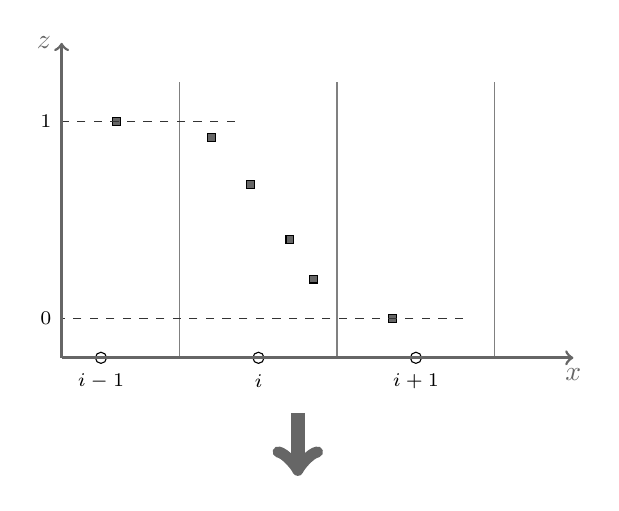
\begin{tikzpicture}[domain=1:5]
	\node (A1) [circle,draw,inner sep=0.5mm]  at (0.5,0){}; 
	%\node (A2) [circle,draw,inner sep=0.5mm]  at (1,0){}; 
	%\node (A4) [circle,draw,inner sep=0.5mm]  at (2,0){}; 
	\node (A5) [circle,draw,inner sep=0.5mm]  at (2.5,0){}; 
	%\node (A6) [circle,draw,inner sep=0.5mm]  at (3,0){}; 
	%\node (A8) [circle,draw,inner sep=0.5mm]  at (4.,0){}; 
	\node (A9) [circle,draw,inner sep=0.5mm]  at (4.5,0){}; 
     
	\node at (1.9,2.8)[rectangle,draw,fill=black!60,inner sep=0.5mm]{};
	\node at (2.4,2.2)[rectangle,draw,fill=black!60,inner sep=0.5mm]{};
	\node at (0.7,3)[rectangle,draw,fill=black!60,inner sep=0.5mm]{};
	\node at (3.2,1.0)[rectangle,draw,fill=black!60,inner sep=0.5mm]{};
	\node at (2.9,1.5)[rectangle,draw,fill=black!60,inner sep=0.5mm]{};
	\node at (4.2,0.5)[rectangle,draw,fill=black!60,inner sep=0.5mm]{};

	%\node (A10) [circle,draw,inner sep=0.5mm]  at (5.,0){}; 
     \draw [line width=0.5pt,color=black!50,] (1.5,0)--(1.5,3.5);
     \draw [line width=0.5pt,color=black!50,] (3.5,0)--(3.5,3.5);
     \draw [line width=0.5pt,color=black!50,] (5.5,0)--(5.5,3.5);
     \draw [line width=0.5pt,color=black!80,dashed] (2.2,3)--(0,3);
     \draw [line width=0.5pt,color=black!80,dashed] (5.1,0.5)--(0,0.5);
%     \draw [line width=0.5pt,color=black!80,dashed] (2,2.51)--(0,2.51);
%     \draw [line width=0.5pt,color=black!80,dashed] (3,3.0)--(0,3.0);
%     \draw [line width=0.5pt,color=black!80,dashed] (4,2.73)--(0,2.73);
%     \draw [line width=0.5pt,color=black!80,dashed] (5,1.83)--(0,1.83);
\draw  [->,line width=1pt,color=black!60](0,0)--(6.5,0) node [anchor=north] {$x$};
 \draw [->,line width=1pt,color=black!60](0,0) -- (0,4) node [anchor=east] {$z$};
 \node at (-0.2,0.5) {\scriptsize $0$};
 \node at (-0.2,3) {\scriptsize $1$};
 \node at (2.5,-0.3) {\scriptsize $i$};
 \node at (4.5,-0.3) {\scriptsize $i+1$};
 \node at (0.5,-0.3) {\scriptsize $i-1$};
 %\draw [line width=0.6pt,color=red!60!black!40] (3.2-0.15,0.5-0.1)--(3.2+0.15,0.5+0.1);
 %\draw [line width=0.6pt,color=red!60!black!40] (3.2+0.15,0.5-0.1)--(3.2-0.15,0.5+0.1);
 %\draw [line width=0.6pt,color=red!60!black!40] (2.4+0.15,3-0.1)--(2.4-0.15,3+0.1);
 %\draw [line width=0.6pt,color=red!60!black!40] (2.4-0.15,3-0.1)--(2.4+0.15,3+0.1);

 %\draw [line width=0.6pt,color=red!60!black!40] (1.9+0.15,3-0.1)--(1.9-0.15,3+0.1);
 %\draw [line width=0.6pt,color=red!60!black!40] (1.9-0.15,3-0.1)--(1.9+0.15,3+0.1);

 %\draw[line width=1.5pt,color=black!80, dashed](2.9,0)--(2.9,3.5);
 \draw[->,line width=5pt,color=black!60] (3.0,-0.7)--(3.0,-1.5);
\end{tikzpicture}
  \begin{tikzpicture}[domain=1:5]
	\node (A1) [circle,draw,inner sep=0.5mm]  at (0.5,0){}; 
	%\node (A2) [circle,draw,inner sep=0.5mm]  at (1,0){}; 
	%\node (A4) [circle,draw,inner sep=0.5mm]  at (2,0){}; 
	\node (A5) [circle,draw,inner sep=0.5mm]  at (2.5,0){}; 
	%\node (A6) [circle,draw,inner sep=0.5mm]  at (3,0){}; 
	%\node (A8) [circle,draw,inner sep=0.5mm]  at (4.,0){}; 
	\node (A9) [circle,draw,inner sep=0.5mm]  at (4.5,0){}; 
     
%	\node at (1.9,2.8)[rectangle,draw,fill=black!60,inner sep=0.5mm]{};
%	\node at (2.4,2.2)[rectangle,draw,fill=black!60,inner sep=0.5mm]{};
	\node at (0.7,3)[rectangle,draw,fill=black!60,inner sep=0.5mm]{};
	\node at (2.7,1.5)[rectangle,draw,fill=red!60!black!80,inner sep=0.5mm]{};
%	\node at (2.9,1.5)[rectangle,draw,fill=black!60,inner sep=0.5mm]{};
	\node at (4.2,0.5)[rectangle,draw,fill=black!60,inner sep=0.5mm]{};

	%\node (A10) [circle,draw,inner sep=0.5mm]  at (5.,0){}; 
     \draw [line width=0.5pt,color=black!50,] (1.5,0)--(1.5,3.5);
     \draw [line width=0.5pt,color=black!50,] (3.5,0)--(3.5,3.5);
     \draw [line width=0.5pt,color=black!50,] (5.5,0)--(5.5,3.5);
     \draw [line width=0.5pt,color=black!80,dashed] (2.2,3)--(0,3);
     \draw [line width=0.5pt,color=black!80,dashed] (5.1,0.5)--(0,0.5);
%     \draw [line width=0.5pt,color=black!80,dashed] (2,2.51)--(0,2.51);
%     \draw [line width=0.5pt,color=black!80,dashed] (3,3.0)--(0,3.0);
%     \draw [line width=0.5pt,color=black!80,dashed] (4,2.73)--(0,2.73);
%     \draw [line width=0.5pt,color=black!80,dashed] (5,1.83)--(0,1.83);
\draw  [->,line width=1pt,color=black!60](0,0)--(6.5,0) node [anchor=north] {$x$};
 \draw [->,line width=1pt,color=black!60](0,0) -- (0,4) node [anchor=east] {$z$};
 \node at (-0.2,0.5) {\scriptsize $0$};
 \node at (-0.2,3) {\scriptsize $1$};
 \node at (2.5,-0.3) {\scriptsize $i$};
 \node at (4.5,-0.3) {\scriptsize $i+1$};
 \node at (0.5,-0.3) {\scriptsize $i-1$};
 \node at (2.7,1.7) {\scriptsize $P$};
 %\draw [line width=0.6pt,color=red!60!black!40] (3.2-0.15,0.5-0.1)--(3.2+0.15,0.5+0.1);
 %\draw [line width=0.6pt,color=red!60!black!40] (3.2+0.15,0.5-0.1)--(3.2-0.15,0.5+0.1);
 %\draw [line width=0.6pt,color=red!60!black!40] (2.4+0.15,3-0.1)--(2.4-0.15,3+0.1);
 %\draw [line width=0.6pt,color=red!60!black!40] (2.4-0.15,3-0.1)--(2.4+0.15,3+0.1);

 %\draw [line width=0.6pt,color=red!60!black!40] (1.9+0.15,3-0.1)--(1.9-0.15,3+0.1);
 %\draw [line width=0.6pt,color=red!60!black!40] (1.9-0.15,3-0.1)--(1.9+0.15,3+0.1);

 %\draw[line width=1.5pt,color=black!80, dashed](2.9,0)--(2.9,3.5);
\end{tikzpicture}
\caption{��ɢ��������е�Ԫ�����ȥ����һάʾ��ͼ}
\label{fig:illu_cellpoint_choose_diffuse}
\end{figure}


